\subparagraph{Задание 4.15}

\textbf{Условие}:
Выполнить команду Animate из меню Run с задержкой 1000 мс.

\textbf{Решение}:

\begin{figure}[!htp]
    \centering
    \begin{minipage}{0.32\textwidth}
        \centering
        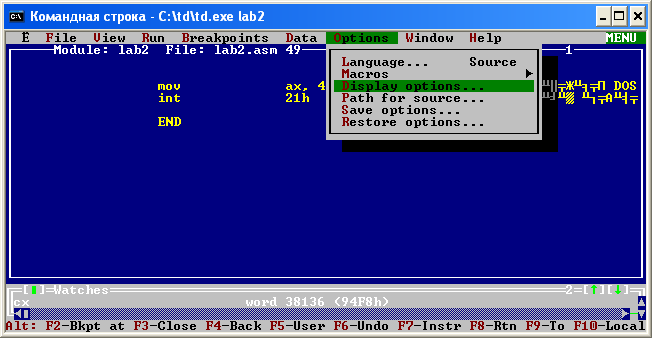
\includegraphics[width=.99\linewidth]
            {../_INCLUDES/task-4-15/1.png}
        \caption{1) }
        \label{fig:task_4_15__1}
    \end{minipage}
    \begin {minipage}{0.32\textwidth}
        \centering
        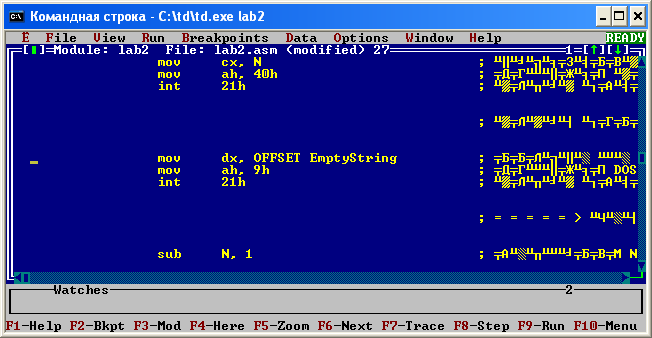
\includegraphics[width=.99\linewidth]
            {../_INCLUDES/task-4-15/2.png}
        \caption{2) }
        \label{fig:task_4_15__2}
    \end{minipage}
    \begin {minipage}{0.32\textwidth}
        \centering
        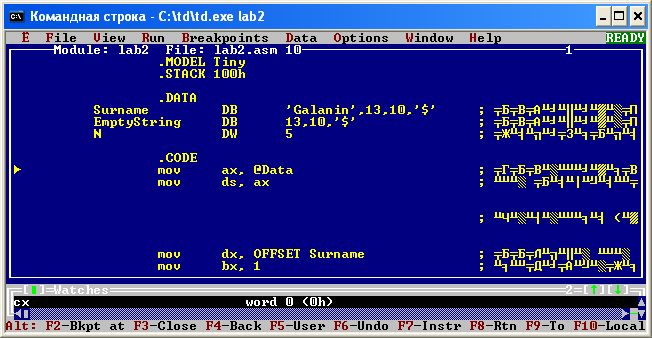
\includegraphics[width=.99\linewidth]
            {../_INCLUDES/task-4-15/3.png}
        \caption{3) }
        \label{fig:task_4_15__3}
    \end{minipage}
\end{figure}

На рисунке~\ref{fig:task_4_15__1} (стр.~\pageref{fig:task_4_15__1})
запущен Turbo Debugger после команды
\textbf{C:\textbackslash\/td\textbackslash\/td.exe lab2}.

Жмем \textbf{F10} - и мы в меню.
Выбираем пункт \textbf{Run}.
Жмём \textbf{Enter}.
Выбираем пункт \textbf{Animate...}.
Жмём \textbf{Enter}.
Рисунок~\ref{fig:task_4_15__2} (стр.~\pageref{fig:task_4_15__2}).

Открылось окно с заданием миллисекунд.
Поле \textbf{Enter animate delay (10ths of sec)} имеет начальное значение \textbf{3}.
Рисунок~\ref{fig:task_4_15__3} (стр.~\pageref{fig:task_4_15__3}).

\begin{figure}[!htp]
    \centering
    \begin{minipage}{0.32\textwidth}
        \centering
        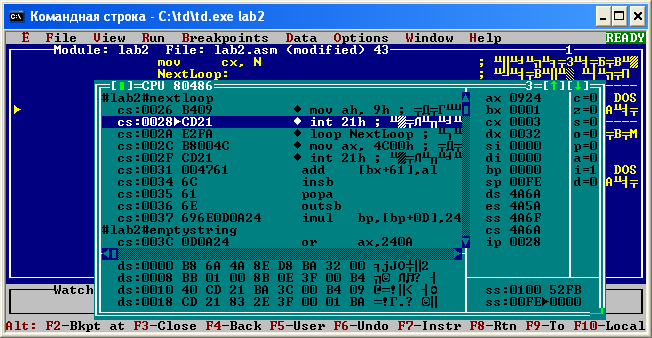
\includegraphics[width=.99\linewidth]
            {../_INCLUDES/task-4-15/4.png}
        \caption{4) }
        \label{fig:task_4_15__4}
    \end{minipage}
    \begin {minipage}{0.32\textwidth}
        \centering
        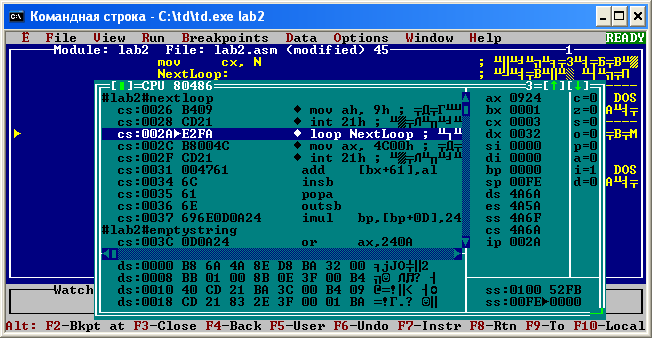
\includegraphics[width=.99\linewidth]
            {../_INCLUDES/task-4-15/5.png}
        \caption{5) }
        \label{fig:task_4_15__5}
    \end{minipage}
    \begin {minipage}{0.32\textwidth}
        \centering
        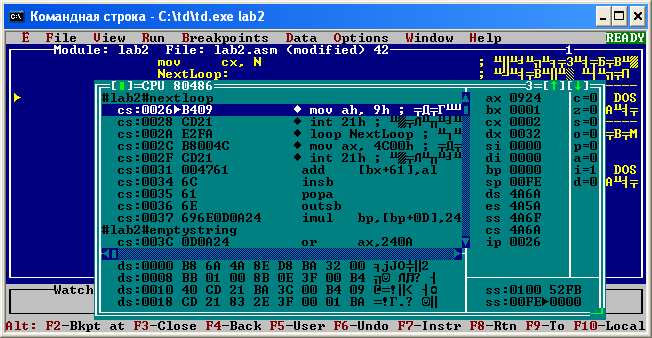
\includegraphics[width=.99\linewidth]
            {../_INCLUDES/task-4-15/6.png}
        \caption{6) }
        \label{fig:task_4_15__6}
    \end{minipage}
\end{figure}

В поле \textbf{Enter animate delay (10ths of sec)} ввожу значение \textbf{1000}.
Рисунок~\ref{fig:task_4_15__4} (стр.~\pageref{fig:task_4_15__4}).

Turbo Debugger выполняет последовательно команду каждую одну секунду.
Рисунок~\ref{fig:task_4_15__5} (стр.~\pageref{fig:task_4_15__5}).

Turbo Debugger сообщает, что программа завершена успешна с кодом 0: \textbf{Terminated, exit code 0}.
Рисунок~\ref{fig:task_4_15__6} (стр.~\pageref{fig:task_4_15__6}).
